\section{Rakefile開発に関するメモ}
\subsection{システムの概要}
卒論編集システム開発時のメモです.

\begin{figure}[htbp]\begin{center}
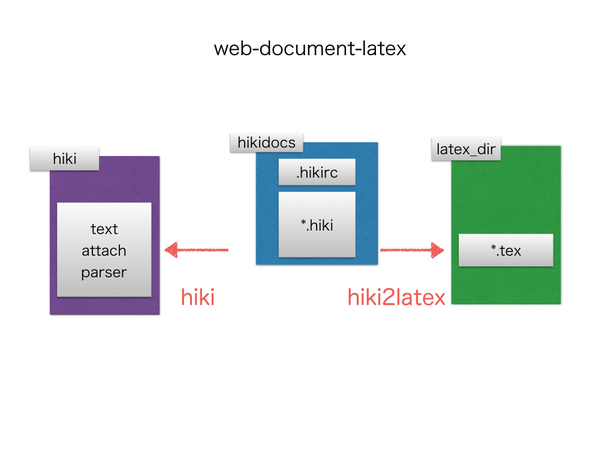
\includegraphics[width=10cm,bb= 0 0 737 453]{../figs/./hikiutils_bob.006.jpeg}
\caption{卒論編集システムの概要}
\label{default}\end{center}\end{figure}
hikiシステムとの同期は,hikiutilsのhikiが下請けしている.
一方,latex\_dirへの出力はlatex2hikiが引き受けている.
フォーマットをいじるときには,基本的に
\begin{description}
\item[hikiへ] hikiがやるので,そのまえにtmp.txtへ写して置換

\item[texへ] latex2hikiからの出力(tmp.txt)を処理してtexへ

\end{description}
で行っている,あるいはおこなう.

\subsection{日本語のcode listings}
日本語のjlistingの挙動がようやく判明しました.listingsでは日本語表示が
ちゃんとなされません.そこで,
\begin{quote}\begin{verbatim}
\usepackage{listings,jlisting}
\end{verbatim}\end{quote}
としています.これで,日本語が含まれたcodeも綺麗に表示してくれます.

\subsection{文献参照のシステム}
latexへ文献参照を渡すために,下記のようなフォーマットでの記述を行う.
\begin{quote}\begin{verbatim}
*{{cite(listings1)}}
*{{cite(listings2)}}

!reference:
:listings1:[[基本的な使い方|http://d.hatena.ne.jp/mallowlabs/20061226/1167137637]]
:listings2:[[listingsの定義の仕方|http://www.ipc.akita-nct.ac.jp/~yamamoto/comp/latex/make_doc/source/source.html]]
\end{verbatim}\end{quote}
これはlatexへの書き換えは単純だが,そのままではhikiシステムでエラーが出る.
hikidocなどをいじるのはあまり筋が良くないので,rake syncにtrapを仕掛ける.

\subsection{rake mk\_toc}
latexが作成するtableofcontentsの実態であるtocファイルからhiki用のtoc.hikiを作成する.

